\documentclass{ctexart}

% Code Block
\usepackage{minted}
\usepackage{xcolor}
\definecolor{LightGray}{gray}{0.9}
\usepackage{listings}
\usepackage{graphicx,color}
\usepackage{booktabs}


% Allows theorem, lemma, and proof
\newtheorem{theorem}{Theorem}[section]
\newtheorem{corollary}{Corollary}[theorem]
\newtheorem{lemma}[theorem]{Lemma}
\usepackage{amsthm}
\newtheorem*{remark}{Remark}
\theoremstyle{definition}
\newtheorem{definition}{Definition}[section]

% Allows overbrace and sidebrace in matrix
\usepackage{xcolor}
\newcommand\overmat[2]{%
  \makebox[0pt][l]{$\smash{\color{white}\overbrace{\phantom{%
    \begin{matrix}#2\end{matrix}}}^{\text{\color{black}#1}}}$}#2}
\newcommand\bovermat[2]{%
  \makebox[0pt][l]{$\smash{\overbrace{\phantom{%
    \begin{matrix}#2\end{matrix}}}^{\text{#1}}}$}#2}
\newcommand\partialphantom{\vphantom{\frac{\partial e_{P,M}}{\partial w_{1,1}}}}

% reference styles
\usepackage{biblatex}
\addbibresource{refs.bib}

% Fancy math symbol font
\usepackage{mathrsfs}

% Change page margin
\usepackage[inner=2.54cm,outer=2.54cm]{geometry}
 
% Set graphic path
\usepackage{graphicx}
\graphicspath{ {images/} }

% Clickable references
\usepackage[unicode]{hyperref}
\hypersetup{
    colorlinks,
    citecolor=black,
    filecolor=black,
    linkcolor=black,
    urlcolor=black
}

% Set Reference styles
\usepackage{biblatex}
\addbibresource{refs.bib}

% Set math tools
\usepackage{amsmath}
\usepackage{amssymb}
\usepackage{empheq}
\usepackage{amssymb}

% Declare atan2 function
\DeclareMathOperator{\atantwo}{atan2}

% Prevent footnotes on second page
\interfootnotelinepenalty=10000
 
 
\title{太阳系建模讨论}
\author{隋东霖}
\date{2020.03.15}

\begin{document}
\maketitle

\section{明确问题}
\label{sec:Introduction}
    本文希望建立的太阳系模型需要满足如下要求:
    \begin{itemize}
        \item 输入:\\
        某一时刻太阳系各天体的坐标、速度与加速度;\\
        可以从JPL公开的星历表\footnote{https://ssd.jpl.nasa.gov/?ephemerides}中得到;
        \item 输出:\\
        未来某一时刻太阳系各天体的坐标、速度与加速度;
        \item 精度:\\
        近似精度;
        \item 表现形式:\\
        数值和动画。
    \end{itemize}
    
    为了便于建模,很多天文学事实都会被忽略。因此,我们做出如下假设:
    \begin{enumerate}
        \item 太阳系模型的坐标原点被设为太阳本身,并且太阳本身保持静止(does not wobble),而并非遵从在天文学领域中常见的J2000.0框架 \footnote{即认为规定TT时2000年1月1日12时的天赤道与二分点为固定的坐标原点} 。
        \item 所有天体都被视作不自转且没有体积的质点,因此周期性的章动等现象都不会被考虑。
        \item 不考虑非行星、非恒星天体。
        \item 不考虑相对论修正。
    \end{enumerate}
    
    要实现满足上述要求的太阳系模型,有两种进路:现实主义(realistic approach)与工具主义(instrumental approach)。现实主义进路通过使用天体真正遵守的物理定律来建立模型,比如把太阳系看做经典的N体问题(N-body problem)。工具主义进度则和机器学习用的拟合模型有些像,通过现有收集到的大量数据拟合出一个多项式或者神经网络用以预测未来数据。这些拟合模型都只有数学意义,本身不代表星系本身的物理意义。这样的模型有古希腊时期发明的Antikythera Mechanism(一种手摇式模拟计算机,用来做天文学预测),或是在预测上更加准确地托勒密体系。本文将简单讨论现实主义进路中的N体问题与工具主义进路中的托勒密体系,以及上述两种进路用Mathematica、MATLAB以及ST语言实现时可能遇到的问题。
    
    \subsection{现实主义进路:作为N体问题}
        通过JPL公开的星历表,我们可以获知任意一个天体在过去历史中的空间坐标位置及其对应的速度和加速度。那么,如果只考虑天体一和天体二,他们的欧氏距离为:
        \begin{equation}
            r_{1,2} = \sqrt{(x_1 - x_2)^2+(y_1 - y_2)^2+(z_1 - z_2)^2}
        \end{equation}
        
        通过使用牛顿第二定律 $\Vec{F}=m\Vec{a}$ 和牛顿万有引力定律
        \begin{equation}
            \Vec{F}=-G\frac{m_1 m_2}{r_{1,2}^2}\hat{r}_{1,2}
        \end{equation}
        我们可以求解出其中一个天体在另一个天体影响下在三个轴方向所受到的力:
        \begin{align}
            \begin{split}
                F_x &= -G\cdot \frac{m_1 m_2}{r_{1,2}^3} \cdot (x_2 - x_1)\\
                F_y &= -G\cdot \frac{m_1 m_2}{r_{1,2}^2}\cdot (y_2 - y_1)\\
                F_z &= -G\cdot \frac{m_1 m_2}{r_{1,2}^3}\cdot (z_2 - z_1)\\
            \end{split}
        \end{align}
        推而广之,我们可以认为,对于一个天体,它所受到的合力可以视为所有天体通过上述这样的二体问题表达式的算术之和,即:
        \begin{align}
            \begin{split}
                \Sigma F_{x,1} &= -(G m_1 m_2) \sum_i \frac{x_i - x_1}{r_{i,1}^3}\;\;\; \forall i \neq 1 \\
                \Sigma F_{y,1} &= -(G m_1 m_2) \sum_i \frac{y_i - y_1}{r_{i,1}^3}\;\;\; \forall i \neq 1 \\
                \Sigma F_{z,1} &= -(G m_1 m_2) \sum_i \frac{z_i - z_1}{r_{i,1}^3}\;\;\; \forall i \neq 1 \\
            \end{split}
        \end{align}
        因为已知天体质量为$m_1$,因此它的加速度可以被求为:
        \begin{align}
            \begin{split}
                 a_{x,1} &= \frac{F_{x,1}}{m_1} \\
                 a_{y,1} &= \frac{F_{y,1}}{m_1} \\
                 a_{z,1} &= \frac{F_{z,1}}{m_1} \\
            \end{split}
        \end{align}
        因此,通过上述原理,可以简单地程序中实现。
        
        \subsubsection{Mathematica实现}
            程序在Mathematica上最容易实现,因为Mathematica有自带的NBodySimulation求解器,配合Graphics3D和Animate函数可以轻松做到模型动画。只需一行代码即可完成(图2)。
            \begin{figure}[h]
                \centering
                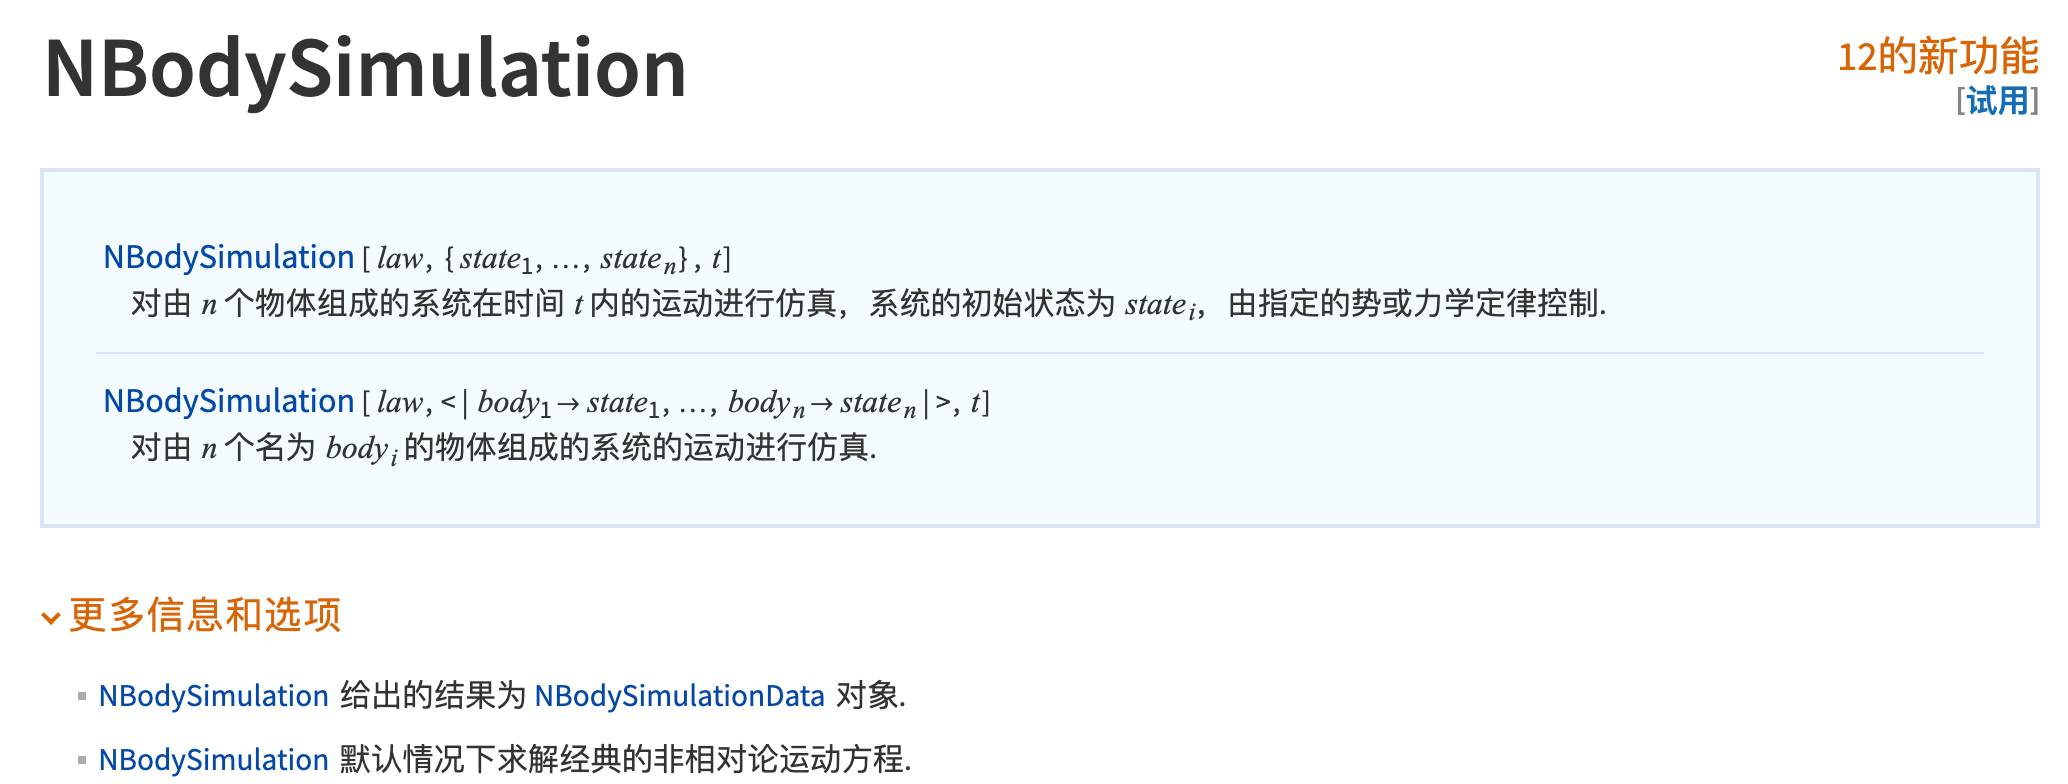
\includegraphics[width=0.9\textwidth]{mathematica_2.png}
                \caption{\label{fig:mathematica_2}NBodySimulation函数}
            \end{figure}
            
            Mathematica的执行速度也很快,甚至可以用这种N体问题的思路来求解小行星带的模拟程序,详情参见\textit{执行小行星的n体仿真} \footnote{https://www.wolfram.com/language/12/astronomy-and-space-science-entities/perform-n-body-simulations-of-asteroids.html.zh?product=language} 。
            
        \clearpage
            
        \begin{figure}[h]
                \centering
                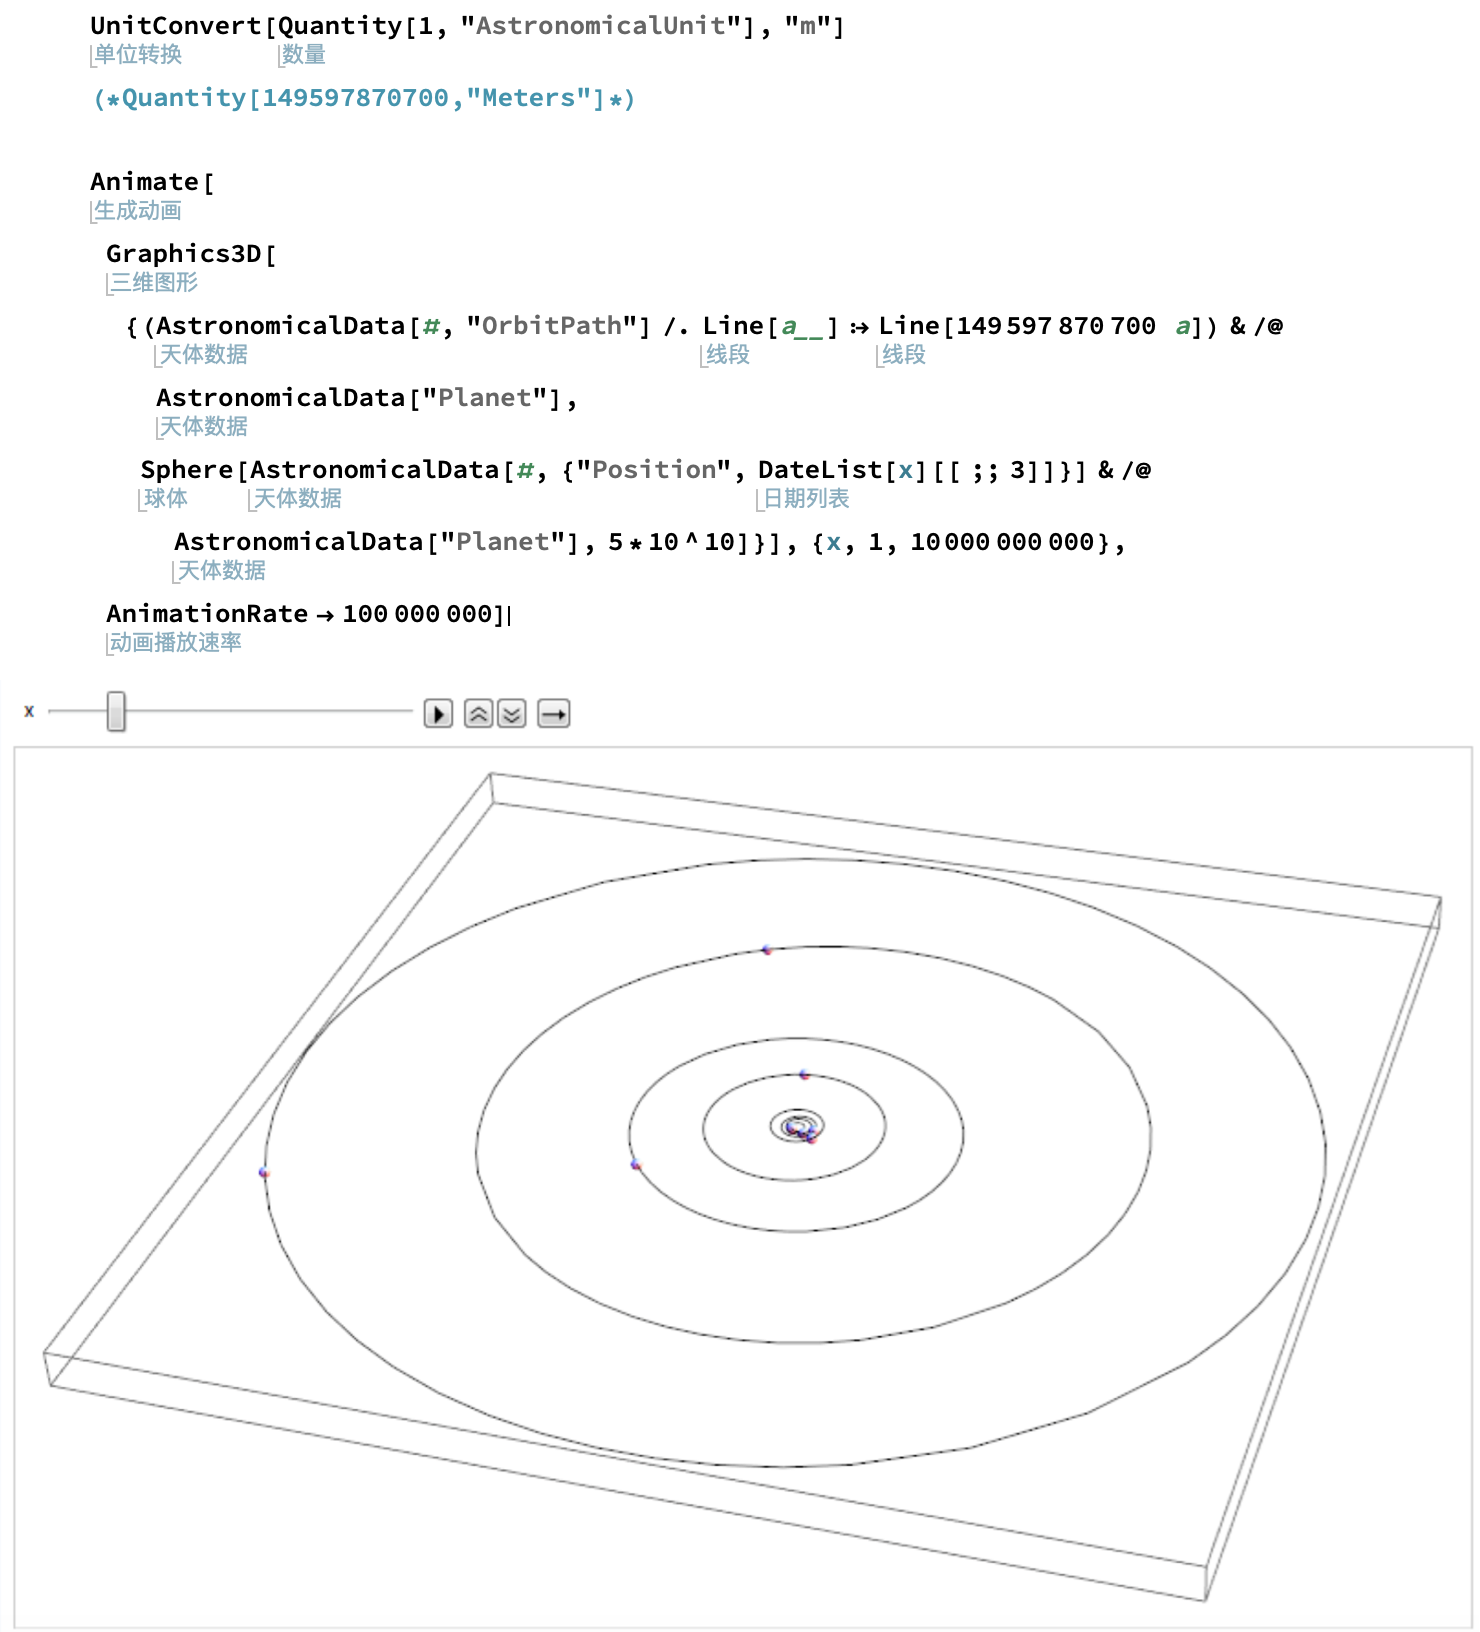
\includegraphics[width=0.60\textwidth]{mathematica_1.png}
                \caption{\label{fig:mathematica_1}图形与动画函数}
        \end{figure}
        
         \subsubsection{MATLAB实现}
            MATLAB实现中的主要困难应该在于动画的表现,因为MATLAB本身适合做静态的plot,目前想到的方法是用openGL作renderer。求解程序本身应该是相当显而易见的,笔者有信心用200-300行左右的代码量来实现整个求解与动画仿真程序。
            
        \subsubsection{ST实现}
            可能遇到的问题:
            \begin{enumerate}
                \item 需要写一个比较方便的数据接口来读取JPL的星历表数据(Mathematica自带星历表);
                \item 需要仔细决定数据的保留位数。就连Mathematica这样自动处理精确度问题的编程语言,如果初始化的时候不适用自带的星历表数据,那么最终计算也会有很大的误差。因此在用ST语言实现的时候,要决定用哪种数据类型;
                \item 需要从零编写求解器,不能用很多方便的数学函数;并且自己编写的话很容易把运算复杂度提升上去;
                \item 不知道怎么用AKENMOTION的Visualization来实现可视化;
            \end{enumerate}
            
        
    \subsection{工具主义进路:托勒密体系}
        托勒密体系是一种地心说体系,通过建立比较复杂的周转圆-均轮系统来拟合实际的天体运动。如果被当作现实主义理论来审视,托勒密体系无疑是错误的,但是从工具主义的角度来看,托勒密体系·改可以提供在精度上不输伽利略体系等日心说理论的预测。因为托勒密体系只需要用圆周齿轮就可以完成建构,所以笔者认为非常适合用ST语言来实现。至于齿轮比的求解过程,既可以使用高中程度的几何知识来手算,也可以使用Mathematica提供的函数来计算。
        \begin{figure}[h]
                \centering
                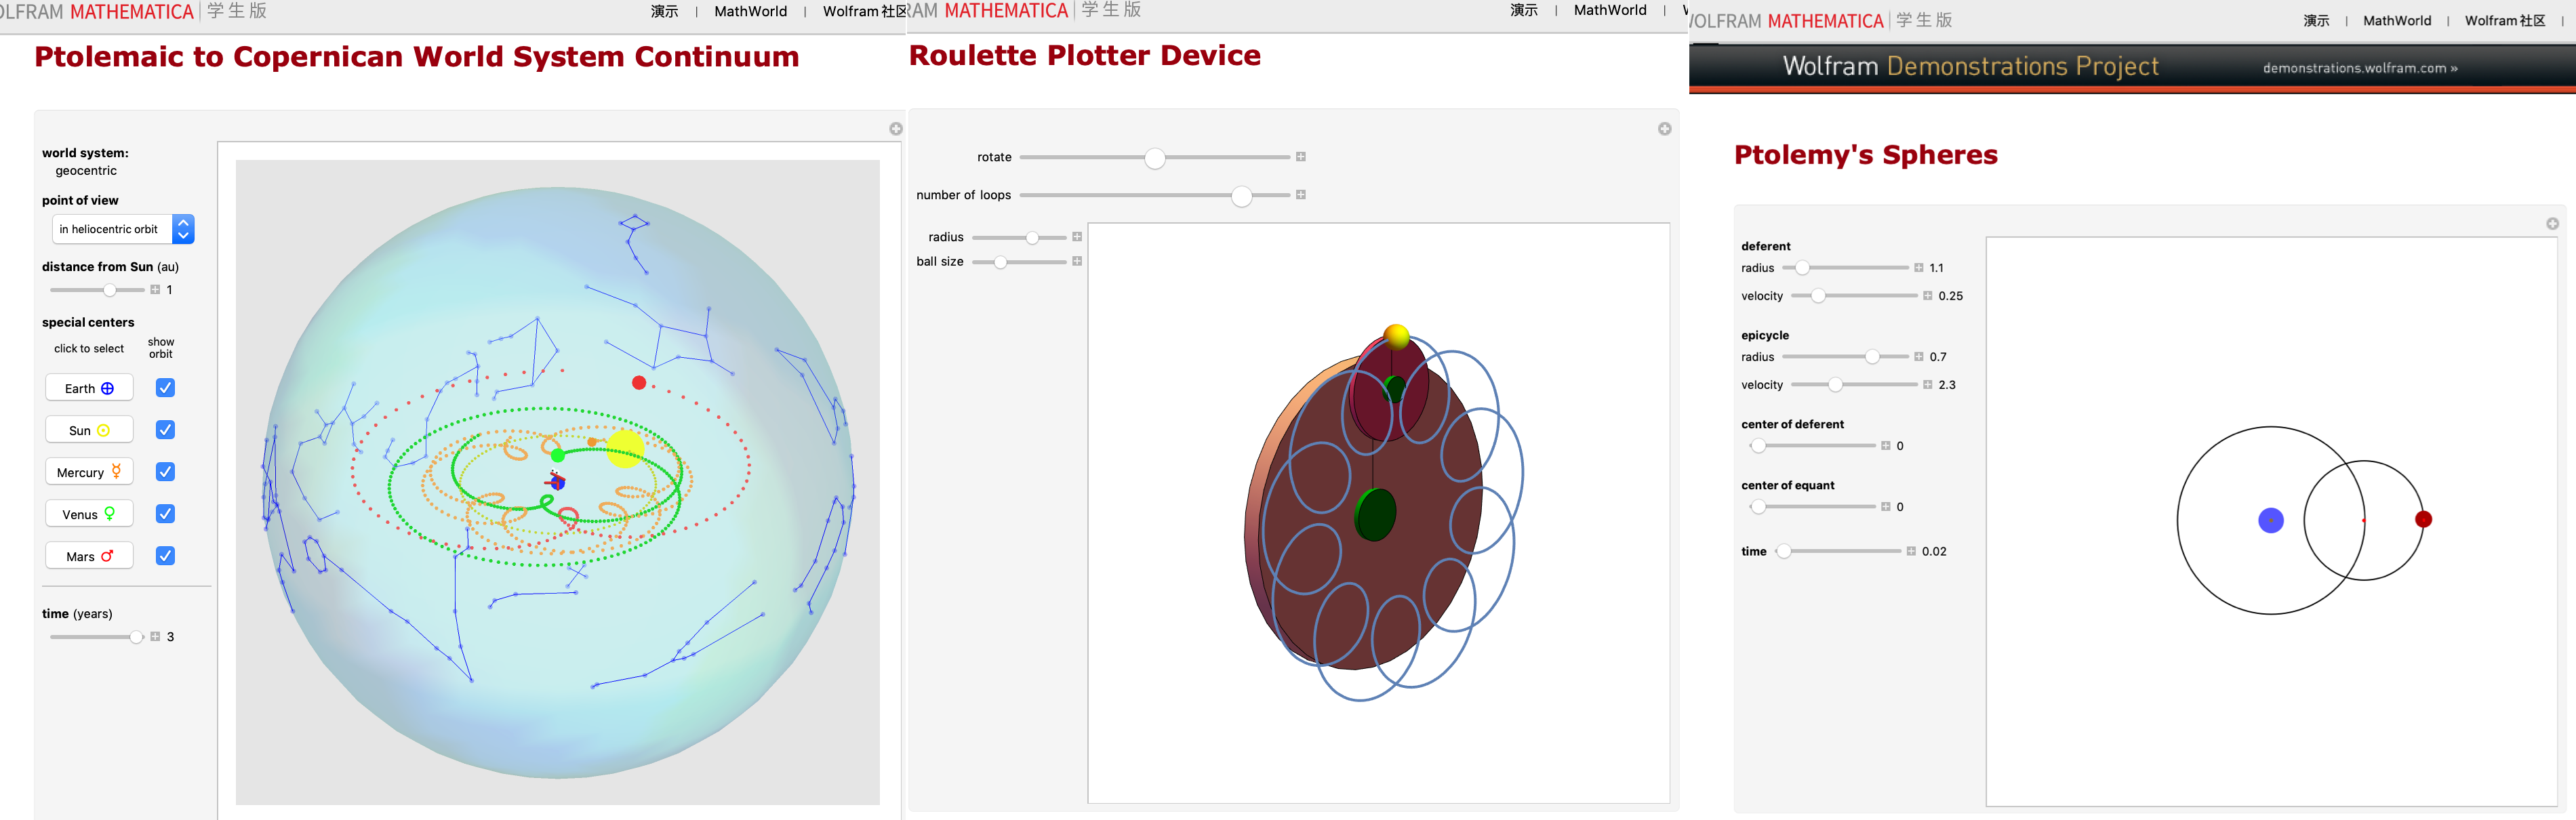
\includegraphics[width=0.80\textwidth]{Ptolemy_3.png}
                \caption{\label{fig:Ptolemy}托勒密体系求解函数}
            \end{figure}
        
\printbibliography[heading=bibintoc, title={参考书目}]
 
\end{document}